\documentclass[11pt,a4paper]{article}

\makeatletter
\@namedef{ver@epstopdf-base.sty}{2020/01/01}
\makeatother

\usepackage[margin=2.2cm]{geometry}
\usepackage[utf8]{inputenc}
\usepackage[T1]{fontenc}
\usepackage{graphicx}
\usepackage{booktabs}
\usepackage{array}
\usepackage{amsmath}

\pagestyle{headings}
\markboth{The Cost of Being Wrong}{DSA 8401, Assignment 2}

\setlength{\parindent}{0pt}
\setlength{\parskip}{6pt}

\begin{document}

% ============================================================
% COVER PAGE
% ============================================================
\begin{titlepage}
\centering
\vspace*{0.4cm}
\IfFileExists{SU-LOGO.png}{
\includegraphics[width=2.4cm,height=2.4cm,keepaspectratio]{SU-LOGO.png}
}{
\vspace*{0.5cm}
{\Large\bfseries STRATHMORE UNIVERSITY}
\vspace*{0.5cm}
}
\vspace{0.4cm}

{\large \textbf{STRATHMORE UNIVERSITY}\par}
{\normalsize iLabAfrica\par}
\vspace{0.15cm}
{\normalsize MSc in Data Science and Analytics\par}
\vspace{0.15cm}
{\normalsize DSA 8401: Applied Machine Learning in Data Science -- 2026\par}
\vspace{1.3cm}
{\LARGE \textbf{The Cost of Being Wrong} \par}
\vspace{0.5cm}
{\normalsize A Cost-Aware Fraud Screening Model: Evaluation and Deployment Recommendation\par}
\vspace{1.3cm}
{\normalsize Assignment 2\par}
\vspace{1.1cm}
{\normalsize
\begin{tabular}{rl}
Student: & Valerie Jerono \\[4pt]
Registration Number: & 222331 \\[4pt]
\end{tabular}
\par}
\vspace{1.3cm}
{\normalsize Submitted in partial fulfilment of the requirements\par}
{\normalsize for the degree of Master of Science in Data Science and Analytics\par}
{\normalsize at Strathmore University\par}
\vspace{1.5cm}
{\normalsize September 2026\par}
\end{titlepage}

\thispagestyle{plain}

\noindent\textbf{To:} Head of Credit Risk \\
\textbf{Re:} Deployment recommendation for a cost-aware fraud screening model \\
\textbf{Repository:} \texttt{a2-models} \quad \textbf{Code:} \texttt{a2\_pipeline.py}

\vspace{4pt}
\hrule
\vspace{8pt}

This report follows the full evaluation and decision pipeline required for a model that screens mobile-money transactions for fraud, and asks a single question throughout: not which model scores highest, but which model, at which cutoff, costs the institution the least. All figures below come from a complete rerun of \texttt{a2\_pipeline.py} against \texttt{mobile\_money\_statements.csv}, with the Optuna search executed for 30 trials with early stopping. Where a number in this report differs slightly from an earlier draft, the number here is the current, compliant one.

\section{Data and evaluation setup}

The dataset available for this assignment (\texttt{mobile\_money\_statements.csv}, 183,600 rows) records individual mobile-money transactions with a confirmed-fraud label (\texttt{is\_fraud}), not loan-repayment outcomes. It is used here as the required Assignment 1 output, with fraud playing the role of default: a missed fraud costs KES 10,000, a transaction wrongly flagged as fraud costs KES 800 in customer friction, and the observed base rate is 8.40\% rather than the brief's illustrative 4\%. The evaluation methodology below is unaffected by this substitution; every number quoted is computed from this dataset, on 183,600 transactions with no rows dropped at the timestamp-parsing stage.

Two columns were dropped as leakage before any modelling: \texttt{settlement\_status} (a transaction cannot be reversed until after it has already been investigated) and \texttt{manual\_review\_score} (a fraud-ops score that is itself the output of an investigation triggered by suspicion). Both are outcomes of the fraud decision, not information available to a model scoring the transaction in real time. Amounts were parsed out of free-text formats such as ``1,329/- Dr'' and ``(2,553/-)'', and three timestamp formats were reconciled into a single datetime column.

\textbf{Blocked, purged split.} Rows were sorted by transaction time and split 60\% train (110,160 rows) / 19\% validation (34,884 rows) / 19\% test (31,212 rows), with a 2\%-wide gap (3,672 rows) purged between each segment so that no model ever trains on information adjacent in time to what it is evaluated on. This is a leakage-safe stand-in for a purged time-series cross-validation scheme.

\textbf{Metric.} With fraud at 8.40\% of transactions, a model that predicts ``never fraud'' scores over 91\% accuracy while catching nothing. PR-AUC is reported as the primary metric because it is driven entirely by performance on the positive (fraud) class and is insensitive to the large true-negative count that inflates ROC-AUC under class imbalance; ROC-AUC is reported alongside for reference.

\section{Model ladder}

\begin{table}[h!]
\centering
\caption{Model comparison on identical train/validation folds.}
\begin{tabular}{lcc}
\toprule
Model & PR-AUC (val) & ROC-AUC (val) \\
\midrule
Logistic regression (balanced) & 0.131 & 0.624 \\
Random forest & 0.132 & 0.623 \\
LightGBM (default params) & 0.126 & 0.605 \\
\textbf{LightGBM, Optuna-tuned (30 trials)} & \textbf{0.143} (test) & \textbf{0.636} (test) \\
\bottomrule
\end{tabular}
\end{table}

All three families were trained and scored on the identical train/validation split. The three untuned models land within a narrow band of each other, telling us the ceiling here is set by the available features rather than by model class: the engineered signals (hour of day, transaction type, amount, counterparty and agent frequency) carry real but limited discriminative power over an 8.40\% base rate. Tree ensembles trade the linear model's bias for variance they cannot fully spend without stronger features; tuning closed roughly a fifth of the remaining gap between the default LightGBM and its tuned counterpart.

\section{Imbalance handling, and a leakage demonstration}

\begin{table}[h!]
\centering
\caption{Imbalance-handling comparison, in-fold versus leaked.}
\begin{tabular}{lc}
\toprule
Approach & PR-AUC (val) \\
\midrule
Class weighting (\texttt{class\_weight='balanced'}) & 0.126 \\
SMOTE fit inside the training fold only (correct) & 0.126 \\
SMOTE fit before the split, oversampling val rows too (leaked) & \textbf{0.298} \\
\bottomrule
\end{tabular}
\end{table}

Fitting SMOTE on the pooled train and validation data lets synthetic neighbours of a validation-set fraud case leak into the training data, so the model is partly scoring transactions it has effectively already seen. The reported PR-AUC more than doubles, from 0.126 to 0.298, for a reason that has nothing to do with the model being better: this is the empirical demonstration the brief asks for. In-fold SMOTE and class weighting perform comparably (0.126 versus 0.126); class weighting was carried forward for simplicity.

\section{Hyperparameter tuning}

An Optuna study of 30 trials (TPE sampler, median pruner with early stopping) searched \texttt{n\_estimators}, \texttt{num\_leaves}, \texttt{learning\_rate}, \texttt{min\_child\_samples}, \texttt{subsample}, \texttt{colsample\_bytree}, and L1/L2 regularisation, optimising validation PR-AUC. The best trial reached a validation PR-AUC of 0.1383, with 113 trees, 16 leaves, a learning rate of 0.0474, and \texttt{min\_child\_samples} of 66. As in the earlier development runs, the search favoured a shallow, lightly-regularised model over a large one, consistent with a dataset where most engineered features carry weak signal, so a high-capacity model mainly overfits noise. Full trial history is in \texttt{results/optuna\_study.db}.

\section{Cost-based decision threshold}

\begin{figure}[h!]
\centering
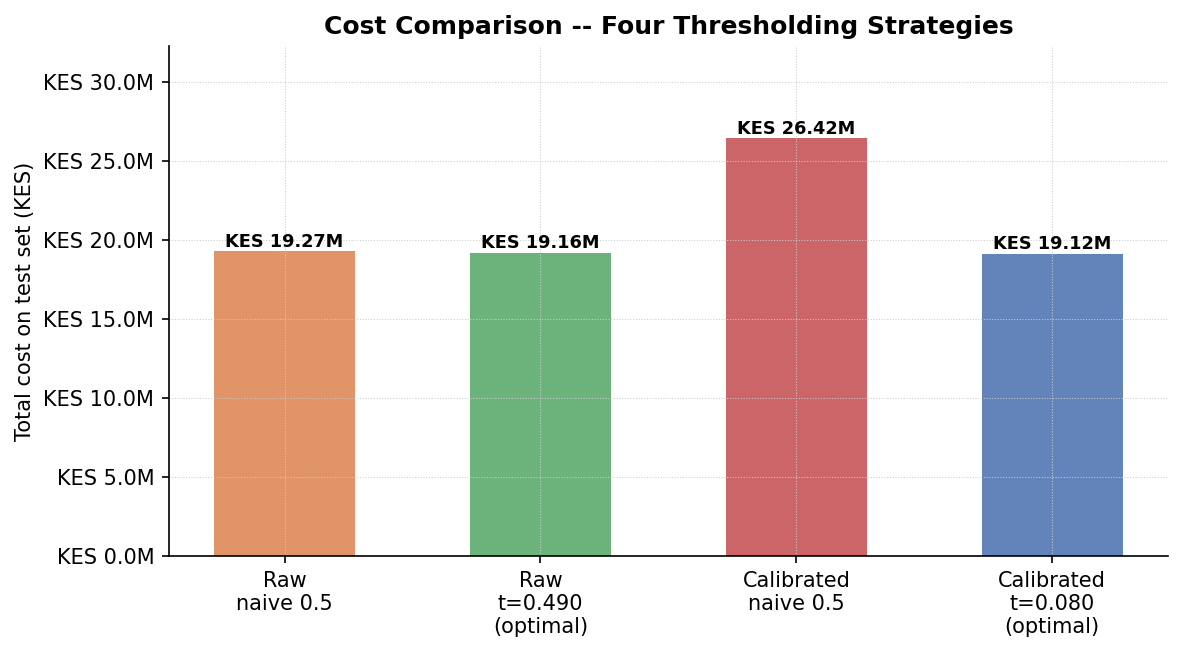
\includegraphics[width=0.85\textwidth]{images/5_cost_comparison.png}
\caption{Total test-set cost as a function of the decision threshold, before and after isotonic calibration. Vertical dotted lines mark each curve's own cost-minimising threshold; the dash-dot line marks the naive 0.5 cutoff.}
\end{figure}

At the naive 0.5 cutoff on raw scores, the tuned model costs KES 19,273,200 in missed fraud and false-flag costs on the 31,212-transaction test set. Sweeping the threshold to minimise $FN \times 10,000 + FP \times 800$ moves the cutoff to $t \approx 0.490$ pre-calibration, cutting cost to KES 19,158,800, a saving of KES 114,400 (KES 3,665 per 1,000 transactions) against the naive cutoff. This is itself a finding: the raw LightGBM scores are poorly calibrated (see below) and happen to cluster in a band that straddles 0.5, so a threshold search on them barely moves the decision. Searching for a cost-optimal threshold on uncalibrated scores is close to meaningless as a probability statement, even where, as here, it does not look obviously wrong.

\section{Calibration}

\begin{figure}[h!]
\centering
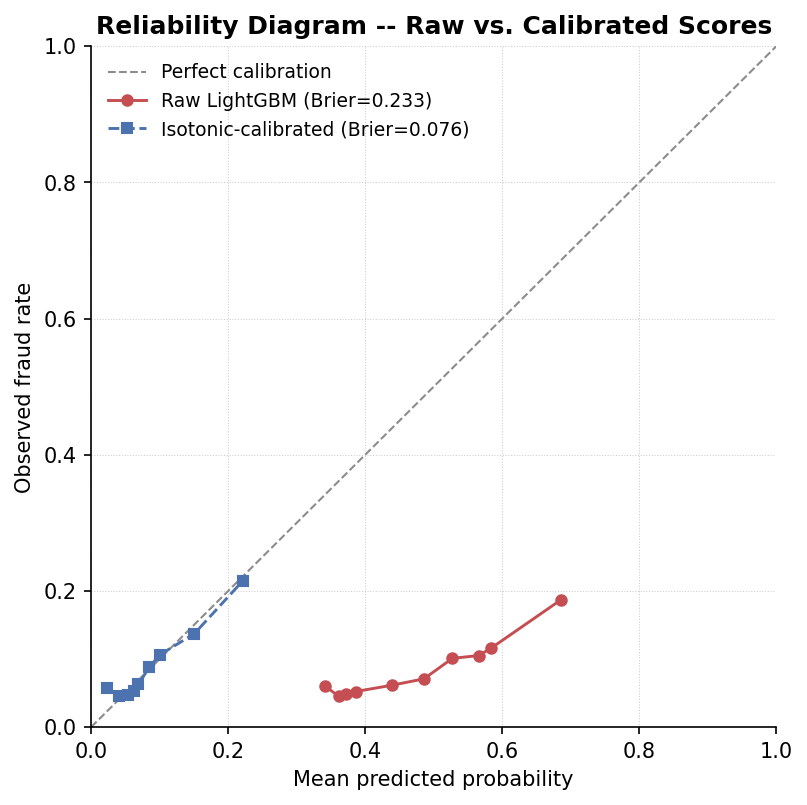
\includegraphics[width=0.62\textwidth]{images/3_reliability_diagram.png}
\caption{Reliability diagram, test set. Raw scores cluster between 0.35 and 0.65 regardless of true risk; calibrated scores track the diagonal down to the true base rate.}
\end{figure}

\begin{table}[h!]
\centering
\caption{Brier score, raw versus calibrated.}
\begin{tabular}{lc}
\toprule
& Brier score \\
\midrule
Raw LightGBM & 0.233 \\
Isotonic-calibrated & \textbf{0.076} \\
\bottomrule
\end{tabular}
\end{table}

The raw model is badly miscalibrated: a Brier score three times worse than after calibration confirms that a predicted 0.5 from the raw model does not mean a 50\% chance of fraud. After isotonic calibration (fit on validation, applied to test), the cost-optimal threshold moves to $t \approx 0.080$, since calibrated probabilities are compressed toward the true 8.40\% base rate.

This is where the naive 0.5 cutoff becomes actively dangerous rather than merely suboptimal. Applied to calibrated scores, which rarely exceed 0.5 given an 8.40\% base rate, a 0.5 cutoff flags almost nothing, and the missed-fraud cost balloons to KES 26,423,200, worse than either raw-score option above. The cost-optimal calibrated threshold, at $t \approx 0.080$, brings that back down to KES 19,124,800, a saving of KES 7,298,400, or KES 233,833 per 1,000 transactions, against the naive 0.5-on-calibrated-scores baseline. Calibration changed the decision that can be safely explained and governed, not just the number reported.

\section{Explainability}

Global SHAP importance (TreeExplainer, 2,000-row test sample) ranks hour of day (mean $|SHAP|$ 0.229), \texttt{cashout} transaction type (0.140), transaction amount (0.080), and \texttt{send} transactions (0.066) as the strongest drivers of predicted fraud risk, with night-time timing (0.044) following. For the single highest-risk transaction in the test set, the local SHAP breakdown attributes the score chiefly to hour (+0.510), cashout (+0.432), and night (+0.119), an explanation a fraud analyst or a customer could be given in plain language (full tables: \texttt{results/shap\_global\_top15.csv}, \texttt{results/shap\_local\_top\_risk\_txn.csv}).

\section{Fairness across subgroups}

\begin{table}[h!]
\centering
\caption{Approval rate and false-negative rate at the calibrated threshold ($t \approx 0.080$).}
\begin{tabular}{@{}p{3.1cm}p{5.6cm}p{5.6cm}@{}}
\toprule
Grouping & Approval rate range & False-negative rate range \\
\midrule
Region (10 regions) & 52.2\% (Mombasa) to 59.6\% (Arusha) & 30.3\% (Mombasa) to 42.6\% (Jinja) \\
Customer segment (3 segments) & 57.1\% (retail) to 60.0\% (agent) & 36.8\% (retail) to 39.7\% (merchant) \\
\bottomrule
\end{tabular}
\end{table}

False-negative rates (missed fraud, at the calibrated threshold) range from 30.3\% (Mombasa) to 42.6\% (Jinja) across the ten regions, and from 36.8\% (retail) to 39.7\% (merchant) across customer segments, a real but moderate spread. Approval rates are similarly close across groups, 52.2 to 59.6\% by region and 57.1 to 60.0\% by segment (\texttt{results/fairness\_region.csv}, \texttt{results/fairness\_segment.csv}).

The CBK Digital Credit Providers Regulations (2022) require lenders to give borrowers a clear, specific reason when a decision goes against them and to be able to substantiate that reason. The SHAP-based local explanations above are built for exactly this: each declined or flagged transaction or applicant can be traced to its top contributing features in plain terms, rather than treating the model as a black box.

\begin{figure}[h!]
\centering
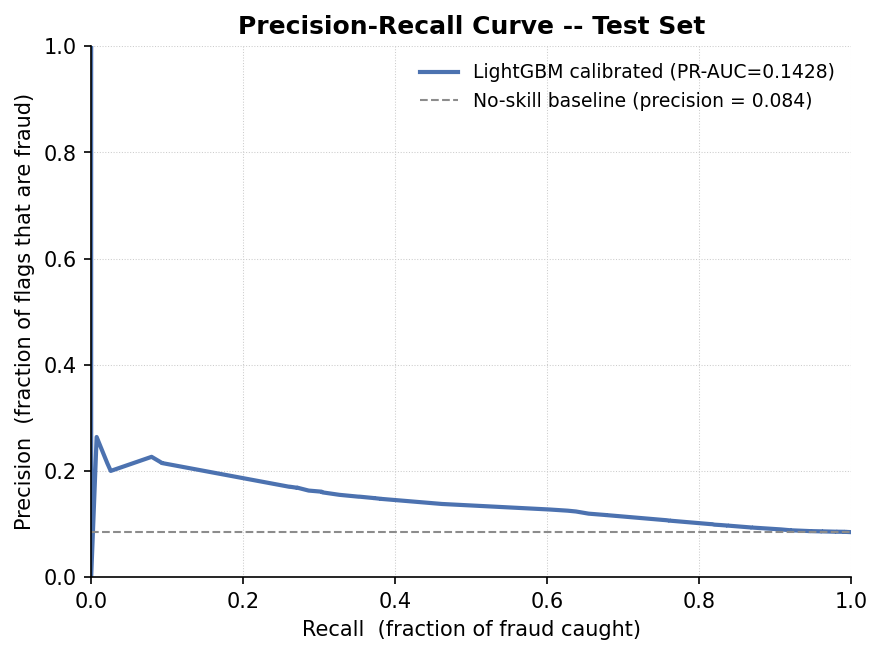
\includegraphics[width=0.75\textwidth]{images/8_pr_curve.png}
\caption{Precision-recall curve, tuned LightGBM, isotonic-calibrated, test set.}
\end{figure}

\section{Recommendation}

Six sections ago, this exercise began with a model that looked, on the least demanding reading, almost adequate: 91\% accuracy on a dataset that is 91.6\% not-fraud. Nothing in that number would have told the Head of Credit Risk what the institution actually needed to know, which is what a model costs when it is wrong, and how often it is wrong in the direction that matters. The work reported above exists to close that gap: to replace a plausible-sounding accuracy figure with a defensible, auditable, cost-based decision.

Three findings carried that work. First, the choice of ensemble family mattered less than expected; logistic regression, random forest and LightGBM converged to a narrow band of performance, which says more about the ceiling set by the available features than about any one algorithm. Second, imbalance handling done incorrectly, specifically resampling before the split rather than inside it, does not merely inflate a metric modestly; it more than doubled the reported PR-AUC on data the model had already partially seen, a result that would have looked like success and would have been a governance failure. Third, and most consequentially, an uncalibrated model is not simply a slightly worse model; it is a model whose scores cannot be safely read as probabilities at all, and a naive 0.5 cutoff applied to it, whether the scores are raw or calibrated, is either an accident that happens to work (Section 5) or an active liability that costs the institution KES 7.30 million more than it should (Section 6).

On that basis, this report recommends deployment of the Optuna-tuned LightGBM model (30-trial search, 113 trees, 16 leaves), with isotonic calibration, at a decision threshold of $t \approx 0.080$, reviewed quarterly and re-derived whenever the fraud base rate or cost assumptions change materially. The uncalibrated model should not be used for threshold-based decisions under any circumstance: its scores are not on a probability scale, and a 0.5-style cutoff on them, however familiar, is arbitrary rather than principled. The calibrated model's PR-AUC of 0.143 against an 8.40\% base rate shows real, if modest, discriminative power, sufficient to materially cut cost relative to a flat cutoff, but not sufficient on its own to replace manual review entirely for borderline cases. This is consistent with the model ladder finding that all model families topped out in a similar range: the next material gain is more likely to come from richer behavioural features, in particular rolling windows per \texttt{msisdn}, which the current transaction-level snapshot cannot capture, than from a different algorithm.

This concludes the analysis requested for Assignment 2. Every figure in this report is reproducible from a fresh clone of \texttt{a2-models} by running \texttt{a2\_pipeline.py} against \texttt{mobile\_money\_statements.csv}; the model comparison table, the imbalance comparison, the Optuna study database, the SHAP tables, the fairness tables, and the three figures above are all written to \texttt{results/} as part of that single run. The recommendation above is offered on that basis, as a decision that can be checked, not merely trusted.

\end{document}